\documentclass{article}
\usepackage[UTF8]{ctex}
\usepackage{geometry}
\usepackage{multirow}
\usepackage{natbib}
\geometry{left=3.18cm,right=3.18cm,top=2.54cm,bottom=2.54cm}
\usepackage{graphicx}
\pagestyle{plain}	
\usepackage{setspace}
\usepackage{enumerate}
\usepackage{caption2}
\usepackage{datetime} %日期
\renewcommand{\today}{\number\year 年 \number\month 月 \number\day 日}
\renewcommand{\captionlabelfont}{\small}
\renewcommand{\captionfont}{\small}
\begin{document}

\begin{figure}
    \centering
    
\includegraphics[width=8cm]{upc.png}

    \label{figupc}
\end{figure}

	\begin{center}
		\quad \\
		\quad \\
		\heiti \fontsize{45}{17} \quad \quad \quad 
		\vskip 1.5cm
		\heiti \zihao{2} 《计算科学导论》个人职业规划
	\end{center}
	\vskip 2.0cm
		
	\begin{quotation}
% 	\begin{center}
		\doublespacing
		
        \zihao{4}\par\setlength\parindent{7em}
		\quad 

		学生姓名:\underline{\qquad  侯鹏辉 \qquad \qquad}

		学\hspace{0.61cm} 号:\underline{\qquad 1907010117\qquad}
		
		专业班级:\underline{\qquad 计科1901 \qquad  }
		
        学\hspace{0.61cm} 院:\underline{计算机科学与技术学院}
% 	\end{center}
		\vskip 1.5cm
		\centering
		\begin{table}[h]
            \centering 
            \zihao{4}
            \begin{tabular}{|c|c|c|c|c|c|c|c|c|}
            % 这里的rl 与表格对应可以看到,姓名是r,右对齐的;学号是l,左对齐的;若想居中,使用c关键字。
                \hline
                \multicolumn{5}{|c|}{分项评价} &\multicolumn{2}{c|}{整体评价}  & 总    分 & 评 阅 教 师\\
                \hline
                自我 & 环境 & 职业 & 实施 & 评估与 & 完整性 & 可行性 &\multirow{2}*{} &\multirow{2}*{}\\
                分析& 分析& 定位 & 方案 & 调整 & 20\% & 20\% & ~&~ \\\            
                10\% & 10\% & 15\% & 15\% & 10\% & &  &~ &~\\
                \cline{1-7} 
                & & & & & & & ~&~ \\
                & & & & & & & ~&~ \\
                \hline      
            \end{tabular}
        \end{table}
		\vskip 2cm
		\today
	\end{quotation}

\thispagestyle{empty}
\newpage
\setcounter{page}{1}
% 在这之前是封面,在这之后是正文
\section{自我分析}
\subsection{自然条件}
性别:男\par
年龄:十九\par
\subsection{身体条件}
身高:170cm左右,体重:56公斤左右,个人感觉个子不高,甚至有些低,因此体重偏轻,所以在高中时想要将体重控制到60公斤左右,但是可能是因为自己时狂吃不胖类型的,所以最高也只是达到58公斤。血压:之前是正常偏高。\par
\subsection{健康状况}
小时候的我很是活蹦乱跳,所以那时为我以后的健康条件打下基础,因此再后来已经不怎么运动的情况下仍然吃得消,不过也不是我不想动,只是后来其他事情太多,便很少运动,久而久之,即便我想运动,也动不起来了。过了这个期末,我就好好运动一番。由于父母从小贯彻的小病不吃药,大病少输液的原则,所以我现在也是练就了一身的抗性,从初中到现在生病的次数屈一只手便可数。要说唯一的不足吧,应该就是,经常上火,而且一上火就流鼻血,尤其是冬天,显得尤为明显。甚至曾经高中时每天早上晚上必来一次,而早上一般还是我在洗脸的时候,所以总是能弄得满脸血。这可能与我很少喝水有关吧,因为当时感觉学校饮水机的水辣舌头,一度不想喝,以至于最长的一次是连续四天没碰过水杯。不过之后我痛彻的认识到这样的缺点,不得不改掉,最终次数少了起来。不过最近到青岛后,可能是靠海的缘故,空气没那么干燥,不怎么流鼻血了。但我明白,还是得“多喝热水”。\par
\subsection{性格分析}
性格有些偏内向,言语较少,有时喜欢安静,有时又喜欢热闹一些的气氛,同情心强,很想感谢每一个对自己好的人,但是却困惑于怎么行动,总想着改变,却只会有泡影。做选择时总是莫名的心慌,总要提醒一下自己要有依据的选就行了,然而没有依据是还是依旧慌。\par
我感觉性格的形成与原生家庭的关系最大,当然我并非抱怨,客观地分析一下这个的成因。因为家庭条件并不是很好的关系,所以在我出生时,父母总是在外打工,姐姐在市里面上学,只有周天回来。后来便是一个月回来一次。本来这种情况下,很容易造就出来一个叛逆的与人人际关系很好的孩子,然而这时我爸做出了一个明智的选择,买了一台电视,再加之我自己家的新房子是在人数很少的地段,甚至没有邻居,这我可就只能被牢牢的拴住了,很小的时候就喜欢在家看电视,所以即便后来上学后依旧是喜欢在家看电视,这也造成了我到现在为止我也很容易总是以一个旁观的的心态很少,也很难以一个参与者的心态进入。既没有父母的交流,又少有姊妹的交流,与同学们的交流又是比较少。因为交流的少,自然而然的性格偏向于内向化;因为交流的少,懂得大人的事情也就比较少;因为交流的少,像大人一样处理事情的也就很少;因为交流的少,接受新思想的洗礼就很少;因为交流的少,将想法化为行动的能力也偏少;甚至因为交流的少,我连表达自己的情绪都很难。早熟已经是不能的,别人眼中的沉稳,只是因为我没有把握时,还不敢尝试。这可以说是造成我心理性格缺陷的一大诱因,虽说事在人为,但我感觉小时候的熏陶真的很重要。\par 
虽然有失,但也必有得。我的父母对我和我姐是真的好,很少责怪我们,有生以来只有一个是因为我犯了一个重大的道德性错误,挨了一次打,但他们即便那样也不愿下狠手,顶多只是顶着脑袋推几下,没有扇过我们。其他时候,只是顶多说我们几句,就连吵架也很少,至今有过两次。而且他们也会尽量满足我的需求,所以我也是体能在接受范围之内的请求。仍记得小时候放学泡网吧被父母发现后,没几天就有一台电脑降临是的喜悦。真的,父母的教育手段真的很让我感动,我时常会回头想如果我站在父母的立场上,我能不能处理的这样好。真的对父母是实实在在的感到感动,感激,感谢。\par 
\subsection{教育与学习经历}
教育与学习经历:一个没有惊天逆袭,亦没有天才光环,只是一个起起伏伏,缓慢进步的平常人。\par 
没有胎教,没有兴趣班,没有早教。\par
从幼稚园开始时,并没有兴趣学习,我记得很清楚(因为我妈经常说)当时甚至因为我不会写“a”而直接逃课回家不想去学校,然后我就被恐吓了一番,吓得我下午就往学校去,再也没有缺过勤,是一直到高中几乎都是全勤。\par 
升小学时,稀松平常,被分到小班,正常学习,变故就发生在一年级学期末时,我自己都没感觉到是情况下,考了个年级第一,我妈也算是有了话头,自然感觉脸上有光了,我爸应该也是会因此坚定让我们都上学的路途。我也是顺理成章的有了能上学的路。不过我之后的整个小学生活再没考过第一,并不是我骄傲了,因为我不虚荣,不会为了虚荣而努力,每天写完作业,都不多看一会就去玩。更重要的是,对于我来说,好的名次并不吸引我。我连虚荣都不知道是什么。\par 
升初中时,市里的学校对于我们村里的大人都要走后门才可以,我自然没有去,但是我却会比某些去了的更有前途,因为在这里,我没有见识到那么多的花花世界,无趣时只能学习。所以成绩也是还不错。对我影响重大的一件事是初三时的分班(对我们学校,前无古人,后无来者),这是让我初尝高三的滋味,每天学习学到十一点十二点,早上五点就起床。(我说为什么我这么喜欢睡觉)终于,最后中考虽然发挥不太理想,但也比其他大多数人强了。\par 
高中是真的起伏变化史,我就不再多赘述了总得就是,高一懵逼,高二浪,高三苦逼学习,然而也并未感到怎么苦,毕竟我连病痛都很难感到,出了就是困一点。庆幸,我还是能考上中国石油大学(华东)这样的好学校。\par 
\subsection{工作与社会阅历}
本来也是有这样的打算,想要趁着暑假打工一波,没想不到怎么实现,然后我妈记住了,还真给我找来了工作。在工地当技术人员,其实也就是操控电梯,但是有与我妈进行轮换,所以接触到的人有一些,虽然我不善言语,但我妈的交际还可以,他们对我也比较热情,必然有一些人针对,针对就针对了,我也不怎么怕,我在那里也就是勉强保一下我妈的口碑,毕竟对人际的处理并不怎么擅长。找事的话有过一个人,莫得办法,第一时间找老板。这是我唯一能做的。反正也没什么大乱子。\par 
\subsection{知识、技能与经验}
知识的话,高中以下的知识当时还都是杠杠的,现在的话应该还可以。其他的话,对理论天文物理稍感兴趣,其他的有,但是我并不太善于观察自己,以后有机会再补充\par 
技能与经验:虽然并不怎么经历世事,但是出于对于情绪的不敏感性,自己在临危时,可以将各种情绪压下去。清晰地想一下对策,但是思维的急性不够,需要些时间。除了有时候在众人前讲话时,自己稍有些紧张,这个真的只能稍微压一下。其他的已经在暑假工作时有所验证。\par
\subsection{兴趣爱好与特长}
兴趣爱好与特长:小时候很爱跑,爱跳,比较活跃,所以之前跑步是很快,但是由于后来逐渐内向化,加之有些罗圈腿的缘故,还得纠结于跑步姿势,便不怎么跑步了。后来很是喜欢物理,尤其是偏向于理论的天文物理,可是当时学业压力比较大,能接触的时间的较少,初中时还可以每周看一次,但记忆里是真的不佳,每周都得重看。高中时很少看课外书,所以又少有接触,唯一的只有一本霍金先生的《时间简史》,大学时想加入社团,结果据说只是看星星,好像并不怎么感兴趣。便一直放着,还是自己课余时间看吧。\par
\section{环境分析}
\subsection{社会环境分析}
政治形式:现在的政治形势,我感觉是近现代以来最好的时代,政治比较稳定,国家在世界地位不断上升,国家的发展十分迅速,为我们这新兴时代的产业-IT创造者很大的机会。而且国家的安全性也较强,不会有被人一枪打死的危险。\par 
经济形势:这个更是不用说了,如今国家经济发展极为迅速,稳中向好、长期向好是我国经济没有改变也不会改变的大趋势,能抓上这个机遇的话,势必能不愁几代人的吃穿。\par 
就业形势:好的太好,差的太差。都说了好的太好,那么自己又怎不会成为那个好的人呢?并且我自己也势必会努力成为的。\par 
\subsection{家庭环境分析}
婚姻状况:我爸我妈已婚,未离过,我为结过婚。\par
经济状况:家境只能说很不好,但是在我爸妈的努力下已经成功转型为差不多,我相信在我的努力下,首富不说,幸福爆满的日子还是要过上的。\par
家人期望:虽然父母嘴上不说,但是对于我的期望还是很大的,虽不是什么干一番经天纬地的大事业,但是也得出人头地。\par
\subsection{职业环境分析}
行业现状:好的很可以,而差着云云。计算机专业毕业生人数要多于其它专业的学生。尽管近几年IT行业陷入低迷、计算机专业人数在其它所有专业中的人数最多,但与其它专业相比,社会和用人单位对计算机专业毕业生的需求量也较大,供求矛盾并不突出。且就业率发展平稳,但薪酬水平有所下降。\par 
职业:职业要求的话,对于本科生来说,专业课学会变可以了,但是我不会局限于此。计算机行业就业前景 ,这个不用担心的,目前前景还是很可以的,不用担心。工作内容,我更喜欢在幕后做研发,但是得先攒够足够资历将其他位置摸清了再去专心搞研发\par 
\subsection{地域与人际环境分析}
工作城市:这个没什么大的要求,可要是对其他地方的了解不怎么深入,没办法定夺,想多转一下,然后最后再找一个适合的地方稳定下来。\par
但是考虑就业前景问题,所以我必须先考虑往大城市先走,因为这种公司游历的几率很大而且有了足够的薪水才可以没有后顾之忧。\par 

\begin{figure}[h]
	\centering
	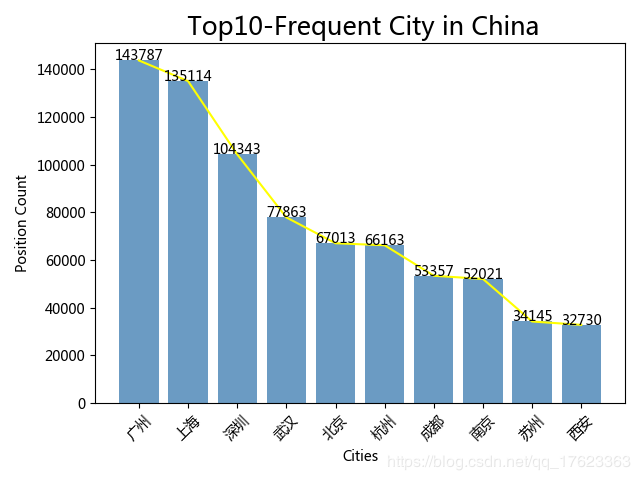
\includegraphics[scale=0.4]{111}
	\caption{计算机专业就职人数排名}
	\label{fig:111}
	\end{figure} \par

据图的话,因为我对北京不太感冒,所以其他几个位置都还是很可以的,可以多加考虑,最终就在青岛也是个不错的选择。\par 
\section{职业定位}
\subsection{行业领域定位与理由}
领域定位:是偏向于技术流的,最终是偏向于幕后。但是我会先将其他领域的知识都了解,这样才能更加完善的开发。
\subsection{职业岗位起点定位与理由}
岗位目标:起点我会凭借自己努力让自己至少比平常人高,争取往精英发展,因为没参加社团的缘故,只报了acm的我有更多的时间将专业可相关的内容理解到更深刻的内容,所以这是我的底气,技术才是硬实力。\par
\subsection{职业目标与可行性分析}
\begin{enumerate}[(1)]
	\item 短期目标:大一大二先将专业知识了解透彻,能够合理运用,大三开始迅速拓展,并合伙接一些项目,以提高自己。大四继续并且思考考研还是工作,可以是两头抓。\par
	\item 长期目标:我想现在一般性的大公司待几年,参加领域如上,在几年后,将进入期待已久的华为公司,传承其精神,并开创其精神,然后寻找合伙人创立新公司,争取为国家的科研尽力,成为一个像倪光南院士的人,而非“美帝良心”钻进钱眼的柳传志。\par
\end{enumerate}

\section{实施方案}
\begin{enumerate}[(1)]
	\item 因为并没有过多的交际的缘故,所以有充分的时间将专业只是学到充分,并不断迁移拓展。\par
	\item 发展人脉对于我有些困难,更多的是,保持现有关系,慢慢的拓展。因为交际人少的缘故,只能依靠自己的可靠吸引更多人。\par
	\item 没事的时候可以去跑跑步,贴近一下大自然,充分享受自然,这是我对我自己的奖励,在自然下,我感觉整个人都有一种自在之感。\par 
\end{enumerate}

\section{评估与调整}
\subsection{评估时间}
可以选择每学期总结一次、每学年评估一次、四年更改调整一次。\par
\subsection{评估内容}
评估内容:根据任务的完成度来做首要评价,若因不可抗拒因素某些未完成,可以根据其他方面的内容来补偿。如果其他方面没有则作为完成。\par
\subsection{调整原则}
由于我制定的计划本本身完成度极高,所以一般不需要做什么改变,到偏差太大时可以作为微调整,但以总目标不变为原则。\par


\end{document}